%%%%%%%%%%%%%%%%%%%%%%%%%%%%%%%%%%%%%%%%%
% Thin Sectioned Essay
% LaTeX Template
% Version 1.0 (3/8/13)
%
% This template has been downloaded from:
% http://www.LaTeXTemplates.com
%
% Original Author:
% Nicolas Diaz (nsdiaz@uc.cl) with extensive modifications by:
% Vel (vel@latextemplates.com)
%
% License:
% CC BY-NC-SA 3.0 (http://creativecommons.org/licenses/by-nc-sa/3.0/)
%
%%%%%%%%%%%%%%%%%%%%%%%%%%%%%%%%%%%%%%%%%

%----------------------------------------------------------------------------------------
%	PACKAGES AND OTHER DOCUMENT CONFIGURATIONS
%----------------------------------------------------------------------------------------

\documentclass[a4paper, 11pt]{article} % Font size (can be 10pt, 11pt or 12pt) and paper size (remove a4paper for US letter paper)

\usepackage[protrusion=true,expansion=true]{microtype} % Better typography
\usepackage{graphicx} % Required for including pictures
\usepackage{wrapfig} % Allows in-line images
\usepackage{changepage}
\usepackage{mathpazo} % Use the Palatino font
\usepackage{amsmath,amsfonts,amsthm,bm}
\usepackage{enumitem}
\usepackage{siunitx}
\usepackage{arydshln}
\usepackage{subfig}
\usepackage[T1]{fontenc} % Required for accented characters
\usepackage[spaces,obeyspaces,hyphens]{url}
\linespread{1.05} % Change line spacing here, Palatino benefits from a slight increase by default

\makeatletter
\renewcommand\@biblabel[1]{\textbf{#1.}} % Change the square brackets for each bibliography item from '[1]' to '1.'
\renewcommand{\@listI}{\itemsep=0pt} % Reduce the space between items in the itemize and enumerate environments and the bibliography

\renewcommand{\maketitle}{ % Customize the title - do not edit title and author name here, see the TITLE block below
\begin{flushright} % Right align
{\LARGE\@title} % Increase the font size of the title

\vspace{50pt} % Some vertical space between the title and author name

{\large\@author} % Author name
\\\@date % Date

\vspace{40pt} % Some vertical space between the author block and abstract
\end{flushright}
}

%----------------------------------------------------------------------------------------
%	TITLE
%----------------------------------------------------------------------------------------

\title{\textbf{Coupling coronary 1D model and porous model}\\ % Title
From concept to implementation on patient data} % Subtitle

\author{\textsc{Lazaros Papamanolis \& Clara Jaquet} \\ Supervised by Irene Vignon-Clementel, Laurent Najman, Hugues Talbot % Author
\\{\textit{INRIA, ESIEE, HeartFlow collaboration}}} % Institution

\date{\today} % Date

%----------------------------------------------------------------------------------------

\begin{document}

\maketitle % Print the title section

%----------------------------------------------------------------------------------------
%	ABSTRACT AND KEYWORDS
%----------------------------------------------------------------------------------------

%\renewcommand{\abstractname}{Summary} % Uncomment to change the name of the abstract to something else

\begin{abstract}
Extrapolation of flow from vasculature to the myocardium tissue requires a complex multi-scale modeling process. We experiment coupling a 1D coronary model with a porous model to compute a physiologically plausible simulation.  

In this report we describe the method, with detailed algorithmn and corresponding codes, current results, and conclusion for future work.
\end{abstract}



\vspace{30pt} % Some vertical space between the abstract and first section
\tableofcontents

%----------------------------------------------------------------------------------------
%	ESSAY BODY
%----------------------------------------------------------------------------------------

\section{Method}

We propose a porous model to simulate blood perfusion, and couple it with the 1D coronary model described in Clara thesis chapter 7. 

In this section we present the porous model, then describe its coupling with the 1D coronary model. We propose a parameterization of the porous model, and provide the detailed algorithm, its command lines and location of scripts to analyze the coupling results.  
 
\subsection{Porous model}
To extend functional analysis into the myocardium with the help of a computational model, here we consider the myocardium as a porous medium. It is a continuous material constituted of 2 phases: a solid phase, or matrix, which contains pores, and a fluid phase, that fills the pores. 

Among the different parameters describing the porous media, the most important ones are porosity $\Phi$ and permeability $\kappa$.
Porosity is defined as the volume fraction of fluid:
\begin{equation}
\Phi = \frac{\texttt{pore volume}}{\texttt{domain volume}}
\end{equation}
It proportionally connects the fluid velocity $v$ and the perfusion velocity (or Darcy velocity) $\bm{\omega}$:
\begin{equation}
\bm{w} = \Phi v 
\end{equation}
The permeability, $\kappa$, is the ability to let fluid go through, corresponding to a conductance factor.
\\
 

The porous model is constructed considering the same assumptions as for the $1D$ coronary model, see Clara thesis manuscript part II, chapter 7, section 1: Assumptions.

To assess implementation of the porous model and its coupling with the $1D$ coronary model of Clara thesis chapter 7, we initiate this work on simulated data with simple geometry.
We define the porous model with the partial differential equation solver $FreeFem++$, verify it, and then compute a coupling with the $1D$ coronary model.

\subsubsection{Porous model equations}
\label{sec:porousmodel}
Because blood is considered incompressible and newtonian fluid, it is governed by Darcy's law in porous media. 
%The perfusion velocity (or Darcy velocity) is defined as :
%\begin{equation}
%\bm{w} = \Phi v 
%\end{equation}
%with $v$ the porous medium velocity and $\Phi$ the volume fraction:
%\begin{equation}
%\Phi = \frac{V_{fluid}}{V_{tissue}}
%\end{equation} 
Darcy's law, a homogenization of Navier-Stokes, is described by a constitutive equation and combined with the fluid mass conservation equation:

\begin{subequations}
\begin{equation}\label{eq:constiDarcy}
\bm{w} + \bm{\kappa} \nabla P = 0
\end{equation}
\begin{equation}\label{eq:conservDarcy}
\nabla \cdot \bm{w} = \beta_{source} \left(P_{source} - P\right) - \beta_{sink} \left(P - P_{sink}\right)
\end{equation}
\end{subequations}
with $\nabla P$ the pressure gradient, $\beta$ a coefficient describing the flow conductance into and out of the tissue, and $P$ the capillary bed pressure. %The latter is related to the fluid velocity via the porosity:


In the constitutive equation, \ref{eq:constiDarcy}, since fluids flow from higher pressure to lower pressure, it follows the pressure drop direction. 

In the fluid mass conservation equation, \ref{eq:conservDarcy},  $\beta_{source}$ represents the inlet through which the blood enters the myocardium with a pressure $P_{source}$, while $\beta_{sink}$ represents the outlet through which blood exits the myocardium with a pressure $P_{sink}$. In terms of physiological meaning, sources and sinks  correspond respectively to arteriole outlets and venous drainage. 

The system is solved for the unknowns Darcy velocity and capillary bed pressure, with pre-estimated parameters.

A verification is designed into a cube geometry to verify the implementation of the porous model is correct. It is presented in the section \ref{sec:results}.

%------------------------------------------------

\subsection{Coupling}

We aim at coupling the $1D$ coronary model of Clara thesis chapter 7 with the porous model of the section \ref{sec:porousmodel}, in both rest and hyperemic conditions.

The vasculature is composed of two dichotomous trees corresponding to the left and right coronaries. Their terminal segment outlets are identified with superscript $T,i$. The interaction between the two models happen at the terminal segment outlets located inside or at the surface of the left ventricle.

The process involves an initialization, followed by iterations coupling the two models. The variable $k$ represents the iteration counter. 
The initialization takes place at $k=0$ and is specific of the condition. It defines the dilation of synthetic segments radii, and porous model parameters, which will all be maintained constant along the iterations.

In the coupling iterations, the resulting pressure of the coronary model at terminal segment ends $P^{T,i}_k$ is used as input for the porous model. The latter calculates flow values at terminal segments, that are used as new inputs for the coronary model, $q^{T,i}_{k+1}$. The convergence is established considering the terminal segment flow values between iteration $k$ and iteration $k+1$. 
\begin{equation}
\frac{\left\lvert q^{T,i}_{k} - q^{T,i}_{k+1} \right\rvert}{q^{T,i}_k} < 1 \% \text{ for all i}
\end{equation}
The figure \ref{fig:couplingloop} illustrates the coupling loop.

\begin{figure}[hbtp]
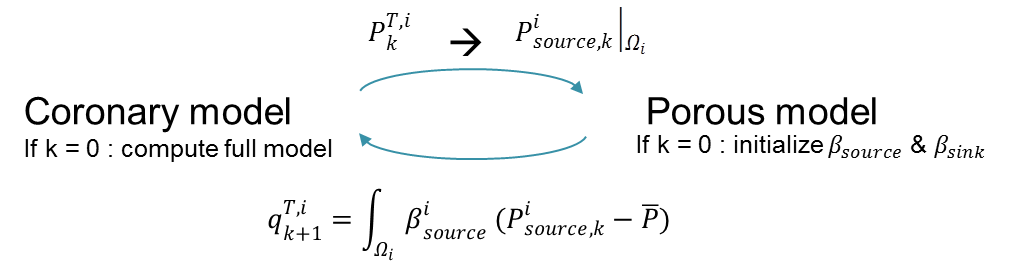
\includegraphics[width = 0.9\textwidth]{Fig/CouplingLoopUpdate.png}
\caption{Illustration of the coupling loop.}
\label{fig:couplingloop}
\end{figure}

We now provide description of the initialization and iterative process of coupling. Further details are given in the pseudo code see section \ref{sec:pseudocode}

\subsubsection{Initialization}
Initialization is made specifically for rest and hyperemic conditions at iteration $k=0$. It involves a first computation of the coronary 1D model, which will be used to estimate the parameters for the porous model.

\paragraph{Coronary model initialization}
The initialization of the coronary model corresponds to the algorithm described in part II, chapter 7 section 2. 
The model is run until convergence specifically for rest or stress condition. It defines synthetic segment dilation in the tree, which will be maintained along iterations, and the first measure of pressure and flow at terminal segments. These two values are used to estimate parameters of the porous model, as detailed in the section \ref{subsec:parameter}.

\subsubsection{Iterations}
For the iteration with $k>0$, the coronary model is simplified into a single solver step.  
The flows $q^{T,i}$ provided by the porous model are used as boundary conditions at the terminal segment ends. The aortic boundary condition is maintained the same as in Clara thesis, meaning $P_{AO} = 93 mmHg$. The solver provides pressure and flow along the vessels. Only the terminal segment end pressures are provided as input for the porous model. 
The porous model is solved with the parameters defined during initialization.




\subsection{Parameterization of the porous model}
\label{subsec:parameter}

To initialize the porous model, we need to estimate the parameters $\kappa$, $\beta_{source}$ and $\beta_{sink}$.\\

\subsection*{Permeability}
The permeability $\kappa$ is estimated as a constant of value \SI{0.002}{\milli\meter\square\per\pascal\per\second} from the literature \cite{chapelle2010poroelastic}. %(\colchg{ I did not found the value in ChapelleVignon 2010, please could you provide me the reference paper for this value?}). 

\subsection*{Coefficient $\beta_{source}$}

The coefficient $\beta_{source}$ is estimated either locally (local $\beta_{source}$) or assumed constant over the myocardium (homogenous $\beta_{source}$).

\subsubsection*{Local $\beta_{source}$}

For each terminal segment end, we estimate $\beta_{source}$ relative to the terminal segment perfusion territory $\Omega_i$ and the terminal segment flow $q^{T,i}$. This perfusion territory is estimated from a weighted Voronoi tessellation (Laguerre Tessellation, see part I, chapter 3, section 3, paragraph \textit{Perfusion territories}). %a smooth version of 

To get a sense of how to estimate $\beta_{source}$, we should consider the physical meaning of the porous model equations.
When considering only the source term, if we integrate the perfusion velocity for each terminal segment end $i$:
\begin{equation}
\int_{\Omega_i}\nabla \cdot \bm{w} = \int_{\Omega_i} \beta_{source} (P_{source} - P)d\Omega
\end{equation}
\begin{equation}
\int_{\partial \Omega_i} \bm{w} \cdot n \approx \beta_{source} (P_{source} - \bar{P}) \Omega_i
\label{eq:intvel}
\end{equation}
The relation defined in equation \ref{eq:intvel} is exactly equal when $P_{source}$ and $\beta_{source}$ are constant over each $\Omega_i$.

The value $P_{source}$ is known, it corresponds to the pressure at the terminal segment end. The pressure drop corresponds to the pressure difference between the terminal segment $i$ and the local region of the porous compartment around this terminal segment (the volume $\Omega_i$).

Considering the left term of equation \ref{eq:intvel} corresponds to the local flow $q^{T,i}$, we can thus estimate $\beta_{source}$ as dimensionally similar to:

%from:
%\begin{equation}
%\beta_{source}^i \sim \frac{q_i}{\Delta P_i \Omega_i}
%\end{equation}
%Which is equivalent to deduce $\beta_{source}$ as inversely proportional to the terminal segment resistance:
\begin{equation}
\beta_{source}^i \sim \frac{1}{R^{T,i} \Omega_i}
\label{eq:estim beta}
\end{equation}

Using the pressure and flow at terminal segment provided by the coronary model, we estimate each $\beta_{source}$ value with:
\begin{equation}
\beta_{source}^i = \frac{q^{T,i}}{(P_{source}^i - \bar{P})\Omega_i}
\end{equation}
For this we use the average capillary pressure $\bar{P} =$\SI{15}{\mmHg} as an estimation of $P$ \cite{chapelle2010poroelastic}.\\

\subsubsection*{Homogeneous $\beta_{source}$}

When assumed homogeneous, the coefficient $\beta_{source}$ is calculated as follows:
\begin{equation}
\beta_{source} = \frac{\sum_{i} q^{T,i}}{(P_{AO} - \bar{P}) \Omega}
\end{equation}

\subsection*{Coefficient $\beta_{sink}$}

The sinks are considered homogeneously distributed over the volume (not explicitly generated), thus we have to determine one single value $\beta_{sink}$. In order to estimate $\beta_{sink}$, we should consider the system behaviour when integrating over the whole myocardium $\Omega_{myo}$. The integral should be equal to 0, since there is as much flow entering as much flow exiting:
\begin{equation}
\int_{\Omega_{myo}} \nabla \cdot \bm{w} = 0
\end{equation}
Thus
\begin{equation}
\int_{\Omega_{myo}} \beta_{source} \left(P_{source} - P\right) = \int_{\Omega_{myo}} \beta_{sink} \left(P - P_{sink}\right)
\end{equation}
Considering $P_{sink}$ as the reference pressure (thus equal to 0) and using the average capillary pressure $\bar{P} =$\SI{15}{\mmHg} as an estimation of $P$ \cite{chapelle2010poroelastic}, we can now estimate the $\beta_{sink}$ value for the whole myocardium: %,\cite{fronek1975microvascular}
\begin{equation}
\beta_{source} \left(P_{AO} - \bar{P}\right) = \beta_{sink} \bar{P} \implies
\beta_{sink} = \frac{\sum_{i} q^{T,i}}{\bar{P} \Omega}
\end{equation}

The parameterisation of the porous medium is done using the \path{beta\_init\_constant.edp} script for the homogenous beta case and the \path{beta\_init.edp} script for the local beta case, written in FreeFem++. 


\subsection{Coupling algorithm}
\label{sec:pseudocode}
In this section we provide pseudo-code, command lines and reference to files used during the coupling process.

\subsubsection{Docker and command lines}
The coupling algorithm combines the porous model code, on the blade, with the 1D coronary model, provided on a docker.\\


Uploading new docker on blade: 
\path{HeartFlow/Coupling/README_Docker.txt} 

Dockers stored on git repo in folder: \path{\HeartFlow\docker}
 
\subsubsection{Pseudo code for coronary model without coupling}
This pseudo-code describes in detail the algorithm expressed in chapter 7 of Clara's thesis.

\begin{enumerate}[label=(\Alph*)]
\item Rest condition (runBaseline=1) \label{itemRest}
\begin{enumerate}[label={\arabic*.}]
\item From synthetic tree: terminal segment radii $r^{T,i}$ \label{itemRestStart}
\item Define initial baseline flows $q^{T,i}_{baseline}$ (read from file \path{baselineFlows.dat}). The file is in principle generated with: $q^{T,i}_{baseline}=Q^{tot}_{rest} \frac{(r^{T,i})^{2.7}}{\sum(r^{T,i})^{2.7}}$
\item Define initial baseline resistance: $R^{T,i} = \frac{P_{AO}}{q^{T,i}_{baseline}}$
\item Define minimum resistance once and fixed for the whole algorithm  (read from file \path{hyperemic_resistances.dat}). The file is in principle generated with: $R^{T,i}_{min} = \frac{1}{4} R^{T,i}$
\item Initialize $q^{T,i} = q^{T,i}_{baseline}$ for boundary condition
\item Run solver with $q^{T,i}$ as boundary condition \label{itemsolv}
\item Compute $R^{T,i}_{sim} = \frac{P^{T,i}_{sim}}{q^{T,i}_{sim}}$. Note: because of BC we have $q^{T,i}_{sim} = q^{T,i}$
\item Check: Main idea is to impose baseline flow if maximum dilation capacity not reached; if it is reached, then reduce flow. So we can end up with a different total rest flow. 

\begin{itemize}
\item If $R^{T,i}_{sim} < R^{T,i}_{min}$ :  \\
full dilation synthetic tree: define new radii $r^{T,i}$ for all upstream synthetic segments using factor $\left(\frac{R^{T,i}}{R_{min}^{T,i}}\right)^{0.25}$ (in principle$ = \sqrt{2}$) and then decrease flow: compute $q_{n+1}^{T,i}=q_n^{T,i} \frac{R_{sim}^{T,i}}{R_{min}^{T,i}} $ (careful when $R_{sim}$ is <0, currently no safeguard so bug!), and go to \ref{itemsolv}
\item If $R^{T,i}_{sim} \geq R^{T,i}_{min}$:\\
Define new radii $r^{T,i}$ for all upstream synthetic segments using factor $\left(\frac{R^{T,i}}{(R_{sim}^{T,i}}\right)^{0.25}$, but same flow and go to \ref{itemsolv}.
\end{itemize}

\item Convergence criteria: \label{itemRestEnd} \\
$max\left( \frac{R_{sim,n+1}^{T,i}-R_{sim,n}^{T,i}}{R_{sim,n+1}^{T,i}} \right) < 1\%$
\end{enumerate}


\item Hyperemic condition (runBaseline=0) \label{itemStress}
\begin{enumerate}[label={\arabic*.}]
\item Define initial baseline flows $q^{T,i}_{baseline}$ (read from file \path{baselineFlows.dat}). The file is in principle generated with: $q^{T,i}_{baseline}=Q^{tot}_{rest} \frac{(r^{T,i})^{2.7}}{\sum(r^{T,i})^{2.7}}$ \label{itemStressStart}
\item Define hyperemic flow as : $q^{T,i}_{stress} = 4 q^{T,i}_{baseline}$
\item Define minimum resistance (read from file \path{hyperemic_resistances.dat}). The file is in principle generated with $R^{T,i}_{min,stress} = \frac{P_{AO}}{q^{T,i}_{stress}}$ (or could also use the rest final resistance and divide it by 4).
\item Compute dilation factor $\left( \frac{R_{baseline}^{T,i}}{R_{min,stress}^{T,i}} \right)^{0.25}$, with $ R_{baseline}^{T,i}= \frac{P_{AO}}{q_{baseline}^{T,i}} $. Dilatation of all synthetic segment radii once with this factor. In general, this factor is 40\%, following Wilson et al. observations \cite{wilson1990effects}. So terminal segments radii are dilated ounce for all:  $r_d^{T,i}$.
\item Run solver with $q^{T,i}_{stress}$ as boundary condition \label{itemsolvstress}
\item Compute $R_{sim,stress}^{T,i}= \frac{P_{sim,stress}^{T,i}}{q_{sim,stress}^{T,i}}$. Note: because of BC we have $q_{sim,stress}^{T,i}=q_{stress}^{T,i}$
\item Check: \label{stressstepcheck}\\

\begin{itemize}
\item If $R_{sim,stress}^{T,i} < R_{min,stress}^{T,i}$, decrease flow: $q_{stress,n+1}^{T,i}=q_{stress,n}^{T,i}  \frac{R_{sim,stress,n}^{T,i}}{R_{min,stress,n}^{T,i}}$, then go to \ref{itemsolvstress}
\item If $R_{sim,stress}^{T,i} \geq R_{min,stress}^{T,i}$, increase flow: $q_{stress,n+1}^{T,i}= q_{stress,n}^{T,i} \frac{R_{sim,stress,n}^{T,i}}{R_{min,stress,n}^{T,i}}$, then go to \ref{itemsolvstress}
\end{itemize}

\item Convergence criteria: \label{itemStressEnd}\\
$max \lvert \frac{ R_{sim,stress}^{T,i} -R_{min,stress}^{T,i}} {R_{min,stress}^{T,i}} \rvert < 1\% $

\end{enumerate}
So in this option, the total flow is no longer controlled in this case, but rather the terminal resistance (by the minimum input resistance value which is based on initial total flow and flow distribution based on initial branch radii, but could also be the rest final resistance and divide it by 4).\\

\item Hyperemic condition by incrementation(runBaseline=0) \label{itemStressIncrem}

In the check step \ref{stressstepcheck}, the factor to modify flow is replaced with:
\begin{equation}
q^{T,i}_{stress, n+1} = q^{T,i}_{stress, n} \frac{\frac{P^{T,i}_{sim, stress, n}}{q^{T,i}_{sim, stress, n}} - R_{min, stress}}{R_{min} + \frac{P_{AO} - P^{T,i}_{sim, stress, n}}{q^{T,i}_{sim, stress, n}}}
\end{equation}

\end{enumerate}


\paragraph*{Input files}
For the 1D coronary model computation the input files are:
\begin{itemize}
\item Description of the synthetic vascular network (segment start coordinate, segment end coordinate, radius): example of filename \path{GRS1_6000_kt6000_s42.txt}
\item Description of synthetic network leaves (coordinate and radius): example of filename \path{Leaves_radii_s42.txt}
\item Description of synthetic tree sources:\path{SourcesForJin7.txt}
\item Segmented vessel description: \path{model.xml}
\item Segmented left ventricle : \path{lv.off}

Note: the 1D coronary model includes computation of the voronoi tessellation

\end{itemize}

\paragraph*{Command lines}
Command lines to run the coronary model:
--inputFlowFile to set the baseline flow
--inputResistanceFile to set the minimum resistance.

\begin{itemize}
\item For rest simulation:
\path{/hfapp/solver/bin/hfsolver-simple-rom-solver --inputFlowFile baselineFlows.dat --runBaseline=1 --inputResistanceFile hyperemic\_resistances.dat -t model.xml}

\item For stress simulation:
\path{/hfapp/solver/bin/hfsolver-simple-rom-solver --inputFlowFile baselineFlows.dat --runBaseline=0 --inputResistanceFile hyperemic\_resistances.dat -t model.xml}

\item For rest simulation with only one iteration:
\path{/hfapp/solver/bin/hfsolver-simple-rom-solver --inputFlowFile baselineFlows.dat --runBaseline=1 --inputResistanceFile hyperemic\_resistances.dat -t model.xml -i 1}

\end{itemize}

\paragraph*{Output files}
The 1D coronary model generates several output files:
\begin{itemize}
\item Result files
\begin{itemize}
\item Hybrid model description: \path{combined_model.xml} or \path{trees_final.xml} 
\item Solutions in hybrid model: \path{VesselTree_ROM_Solved.xml}
\item Log file: \path{coronaryBC.stdout}. Contains the percentage of each territory label.
\item Result of Voronoi tessellation: \path{seedVolumes.dat} or \path{perfusedVolumes.dat}
\end{itemize}

\item Intermediary files
\begin{itemize}
\item Correspondance between leaves coordinates and seed ID: \path{leaves_to_surfaceIds.dat}
\item Strahler order classification, label and morphometry characteristics: \path{treeData.dat} and \path{treeData.vtu}

\end{itemize}
\item Visualization files: if not automatically generated you can call the tool XXXXXX to produce them. 
They can be loaded into paraview.
\begin{itemize}
\item Flow \& pressure solution within segmented vessel geometry: \path{SurfaceMesh_ConnectionMapped.vtu}
\item Flow \& pressure solution within synthetic network geometry: \path{trees.vtk}
\item FFR solution within segmented vessel centerlines : \path{SurfaceMesh_ConnectionMapped_Centerline.vtk}
\item Flow \& pressure \& FFR solution within segmented vessel centerlines and terminal outlets of synthetic network:  \path{SurfaceMesh_ConnectionMapped_Centerline_test.vtu}.

\end{itemize}

\end{itemize}

\subsubsection{Pseudo code of coupling}

The data are provided with a myocardium which is labeled into regions corresponding to a voronoi tessellation algorithm. This  decomposition of the myocardium into convex sub-territories is computed using terminal segment outlets as seeds, with associated speed proportional to their diameters. These regions represent an estimation of a territory $\Omega_i$ perfused by a terminal segment of flow $q^{T,i}$.\\
 
\textbf{Rest condition}\\
\begin{enumerate}[label=(\roman*)]
\item First loop:
\begin{itemize}
\item Run full coronary model until convergence: \ref{itemRest} from \ref{itemRestStart} to \ref{itemRestEnd}. To do so use baseline flows and minimum resistances from \path{baselineFlows.dat} and \path{hyperemic_resistances.dat} files respectively.
\item Initialization of the beta parameters for the porous model using voronoi tessellation territories, terminal segment flows and pressures.
\item Solve the porous model using as input data the data contained in the \path{outputData0.dat} file produced by the 1D coronary model.
\end{itemize}
\item All next loops:
\begin{itemize}
\item Run a single iteration of coronary model: \ref{itemRest} from \ref{itemRestStart} to \ref{itemsolv} with baseline flows provided by porous model (file \path{baselineFlowsK.txt}, where K the number of coupling iteration) and minimum resistance file from Jin. The result provide pressure at leaves (file \path{outputDataK}, where K the number of coupling iteration).
\item Solve the porous model using as input data the data contained in the \path{outputDataK.dat} file produced by the 1D coronary model, where K the number of coupling iteration.
\end{itemize}
\item Convergence criteria\\
$\frac{\left\lvert q^{T,i}_{k} - q^{T,i}_{k+1} \right\rvert}{q^{T,i}_k} < 1 \%$ for all $i$
\end{enumerate}

\textbf{Hyperemic condition}\\
\begin{enumerate}[label=(\roman*)]
\item First loop:
\begin{itemize}
\item Run coronary hyperemic model until convergence: \ref{itemStress} from \ref{itemStressStart} to \ref{itemStressEnd}, using baseline flows and minimum resistances provided by Jin.
\item Initialization of the beta parameters for the porous model using voronoi tessellation territories, terminal segment flows and pressures.
\item Solve the porous model using as input data the data contained in the \path{outputData0.dat} file produced by the 1D coronary model.
\end{itemize}
\item All next loops:
\begin{itemize}
\item Run a single iteration of coronary model in rest condition:  \ref{itemRest} from \ref{itemRestStart} to \ref{itemsolv} with baseline flows provided by porous model (file \path{baselineFlowsK.txt}, where K the number of coupling iteration) and minimum resistance file from Jin. The result provide pressure at leaves (file \path{outputDataK.dat}, where K the number of coupling iteration).
\item Solve the porous model using as input data the data contained in the \path{outputDataK.dat} file produced by the 1D coronary model, where K the number of coupling iteration.
 from \end{itemize}
\item Convergence criteria: same as rest conditions\\
$\frac{\left\lvert q^{T,i}_{k} - q^{T,i}_{k+1} \right\rvert}{q^{T,i}_k} < 1 \%$ for all $i$

\end{enumerate}




\subsection{Post processing}

\subsubsection{Analyze of cfd along the vessels}
To produce analysis such as in the manuscript chapter 8, or appendix E.

See codes in StudyCodes: at the beginning of the code, each substudy is associated the figure number referring to the manuscript:

-morphometry \& cfd:

\path{HeartFlow/SyntheticTreeGeneration_Code/Patient_CCO/Refactor/StudyCodes/PerfSeedStrahlerStudyPressFlowVol.py} 

-correlation between target \& attained flow:

\path{HeartFlow/SyntheticTreeGeneration_Code/Patient_CCO/Refactor/StudyCodes/PerfSynthNetworkStudy.py}

-voronoi territory analysis:

\path{HeartFlow/SyntheticTreeGeneration_Code/Patient_CCO/Refactor/StudyCodes/PerfVoronoiStudy.py}
 
-dilation induced by cfd: 

\path{HeartFlow/SyntheticTreeGeneration_Code/Patient_CCO/Refactor/StudyCodes/ComparingXML.py}


\subsubsection{Analyze of myocardium results with polarmap}
To represent the result into a polarmap, several steps are required.
\begin{itemize}
\item convert the voronoi labeled myocardium mesh to a 3D image (do it only one time for the vascular network, takes 2 weeks at highest resolution: hausd=0.9 and hmax=1.6). Each image voxel contains the value of the corresponding myocardium region label.
\item transfer flow per volume values into this image.
\item then decompose the myocardium flow image into the 17 AHA regions, and project the results in 2D cartography. Note that when producing the polarmap, you can use the same colormap as in perfusion exam if you prefer (see the PolarmapTool on the blade, I commented the lines for this).
\end{itemize}
See code on blade described with \path{/home/jaquetc/ForLazaros/AHACode/README.txt} or on git \path{HeartFlow/Perfusion_Code/CodeForLazaros/README.txt}
Note that the AHA regions are stored for each patient on git, folder:
\path{HeartFlow/PerfusionAHAInputs/}


Then to compare the results with ground-truth exams, you can calculate the correlation as in git code \path{HeartFlow/Perfusion_Code/CorrelateTermFlowWithPerf.py}

\subsubsection{Analyze myocardium results by comparison to literature}
Here we are interested in quantifying global homogeneity and identifying local patterns. This study was computed for flow extrapolated from terminal segments into the myocardium but could potentially be applied to results of the porous model.
The code is on git: \path{HeartFlow/SyntheticTreeGeneration_Code/Patient_CCO/Refactor/StudyCodes/TermFlowStudy.py} 


\section{Results}\label{sec:results}

\subsection{Porous model: Verification test}

A verification is designed into a cube geometry to verify the implementation of the porous model is correct.

For this purpose, we set boundary conditions on the 6 surfaces of the cube as followed:
\begin{itemize}
\item Dirichlet boundary conditions
\begin{itemize}
\item On the face positioned at $x = 0$, named $\Gamma_{in}$, we applied a constant pressure in arbitrary unit: $P_{\Gamma_{in}} = 0$.
\item On the opposite face named $\Gamma_{out}$, we applied a constant pressure $P_{\Gamma_{out}} = 1000$.
\end{itemize}

\item On the four other faces we impose a Neumann boundary condition called "no flux", which induces that the normal velocity of our fluid on those surfaces is zero. Thus our fluid cannot pass through those surfaces, they are considered as hermetic walls.
\end{itemize} 

%\colchg{What values did you use for the parameters $\beta$ and $\kappa$ for this verification test?Do we actually bother since it is arbitrary units?}

We obtained the exact same value between simulated results and analytical solution see figure \ref{fig:verif test}. The visualization of the result is provided in figure \ref{fig:verif visu}.

\begin{figure}[htbp]
\centering
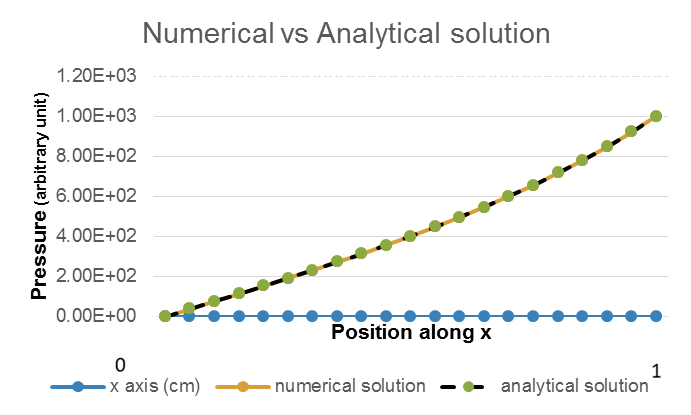
\includegraphics[width=0.6\textwidth]{./Fig/NumVsAnalSol.png}
\caption{Verification test.}
\label{fig:verif test}
\end{figure}

\begin{figure*}[htbp]
\centering
\subfloat{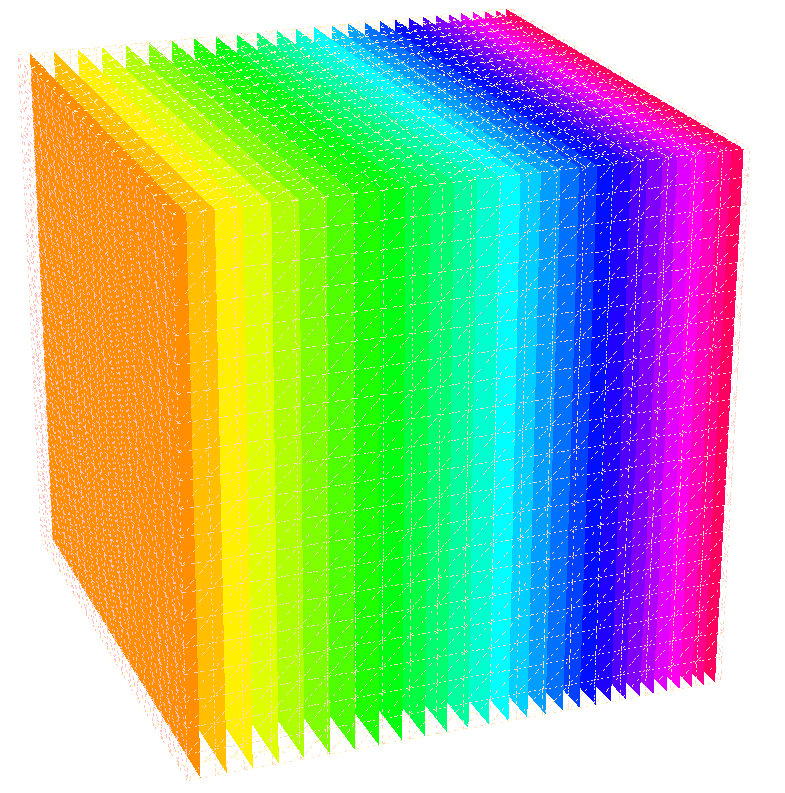
\includegraphics[width=0.6\textwidth]{./Fig/verification_test.PNG}}
\subfloat{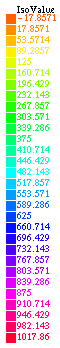
\includegraphics[width=0.11\textwidth]{./Fig/verification_test_iso.PNG}}
\caption{Visual result of verification test.}
\label{fig:verif visu}
\end{figure*}

The porous model implementation is thus verified. 

Note that in our coupling conditions, we will have to set the entering flow through source terms corresponding to the vessel outlets. Also, the exiting flow will be represented by distributed sinks, it will not be a boundary condition anymore.
%Regarding the location of the sink, I believe that every point that does not belong in a boundary surface can be considered as a sink. So you can conceptualize it as if we have a small sink at every point in our system (except of the boundaries), with the same beta or one big sink that affects all points. 

\subsection{Test results on simplified geometry}
In this section, we work with simplified domain geometries: a single bifurcation represents the vascular network, and the shell of a half ellipsoid stands for the left ventricle, see figure \ref{fig:domlab} \protect\subref{dom}. The two terminal segments of the bifurcation, labeled $19$ and $30$, end on the top of the ventricle, on two opposite sides. They are assigned equivalent perfusion territories $\Omega_i$, see figure \ref{fig:domlab} \protect\subref{lab}.\\ 

\begin{figure*}[hbtp]
\subfloat[\label{dom}]{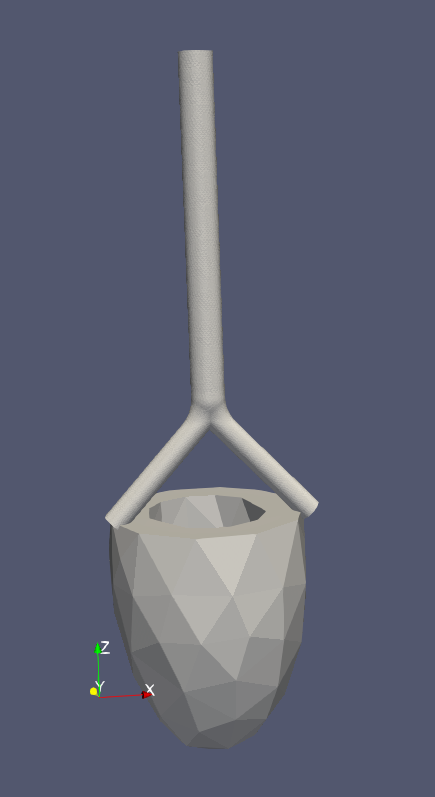
\includegraphics[width = 0.3\textwidth]{Fig/DomainVisualization.png}}
\hspace{0.2cm}
\subfloat{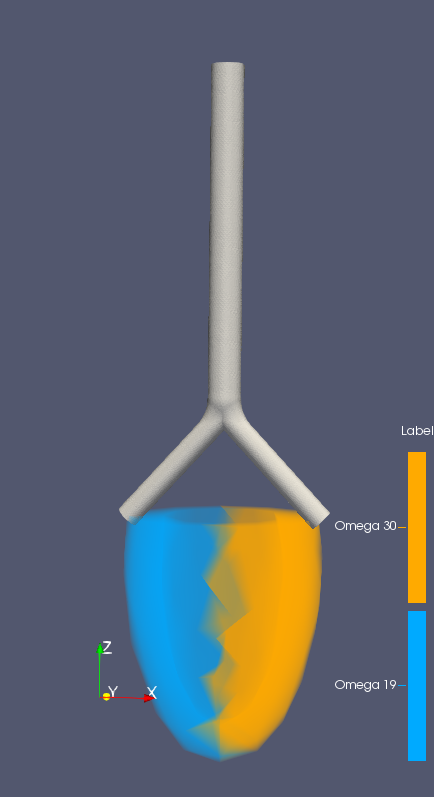
\includegraphics[width = 0.3\textwidth]{Fig/LabelVisualization.png}\label{lab}}
\caption{Visualization of \protect\subref{dom} the simulated coronary and myocardium domains, and \protect\subref{lab} the $\Omega_i$ territory associated to each terminal segment.}
\label{fig:domlab}
\end{figure*}


We study different cases in regards to
\begin{itemize}
\item the condition: either rest or stress
\item the diameter of the terminal vessels: either equal or unequal
\item the parameterisation of the beta coefficients: either calculated, as described in section \ref{subsec:parameter}, or homogeneous. 
\end{itemize}
The varying studies are summarized in the table \ref{tab:defcase}.


\begin{table}[hbtp]
\begin{tabular}{|p{3.5cm}|p{2.5cm}|p{2.5cm}|p{3.5cm}|}
\hline
 & Rest & Stress & Rest with homogeneous $\beta$\\
 \hline
 Equal diameter & case $1$ & case $2$ & case 5\\
 Unequal diameter & case $3$ & case $4$ & case 6\\
 \hline
\end{tabular}
\caption{Definition of the $6$ cases studied.}
\label{tab:defcase}
\end{table}
 
The variable of interests are :
\begin{itemize}
\item the source term pressures, provided by the $1D$ coronary model at each iteration,
\item the flow per terminal vessel, noted $CFD flow$, also output by the $1D$ coronary model at each iteration,
\item the flow per source term, noted $Myo flow$, provided by the porous model at each iteration. 
\end{itemize}

Below we detail parameters and results for cases $1$, $3$, and $6$. Then we summarize results of all cases in the next section.


\subsubsection{Results for case $1$}
The case $1$ corresponds to an equal diameter bifurcation in rest condition.
The table \ref{tab:case1} summarizes the initial parameters.
\begin{figure}[hbtp]
\begin{adjustwidth}{-2.5cm}{}
%\begin{table}[h!]
  \begin{center}
  	\caption{Initial parameters for case 1}
    \label{tab:case1}   
    \begin{tabular}{c|c|c|c|l}  
      \textbf{Parameter} & \multicolumn{2}{c|}{\textbf{Value}} &  \textbf{Units} & \textbf{Description}     \\
      \hline
      $K$           & \multicolumn{2}{c|}{$0.002$}     & \si{mm^{2}.Pa^{-1}.s^{-1}}    & Permeability div$.$ by blood viscosity   \\
      $P_{sink}$     & \multicolumn{2}{c|}{$0$}          & \si{\Pa}     & Venous tree pressure     \\
      $\beta_{sink}$ & \multicolumn{2}{c|}{\SI{10.9844e-5}{}}  & \si{\Pa^{-1}.s^{-1}} & Venous tree beta           \\
      $\bar{P}$     & \multicolumn{2}{c|}{$1999.84$}    & \si{\Pa}      & Average capillary tree pressure    \\      
      \hline
      \hline
                    & \textbf{tv 19} & \textbf{tv 30} &         &                                              \\
      \hline
      $P_{source, k=0}^{i}$       & \SI{12374.4655}{} & \SI{12373.4995}         & Pa      & Source pressure for term$.$ vessel $i$              \\
      $\beta_{source}^{i}$   & \SI{2.0718e-5} & \SI{2.1632e-5}   & \si{Pa^{-1}.s^{-1}} &  Beta of term$.$ vessel $i$  \\
      $q^{T,i}_{k=0}$       & \SI{27.0567} & \SI{27.7974}           & \si{mm^3.s^{-1}}  & Flow rate of term$.$ vessel $i$                  \\               
      $R^{T,i}_{k=0}$       & \SI{457.3523} & \SI{445.1306}               & \si{\Pa  \per\cubic\milli\meter \second}       & Resistance of term$.$ vessel $i$                           \\
      $V_{perf}^{i}$       & \SI{126.5640} & \SI{123.1915}                & \si{\cubic\milli\meter}    & Perfusion volume of term$.$ vessel $i$                \\       
    \end{tabular}
  \end{center}
\end{adjustwidth}
\end{figure}



The figures \ref{fig:flcase1} and \ref{fig:prcase1}\protect\subref{pr1crv} show respectively flow and pressure evolution at terminal segment outlets along iterations. Pressures have converged to their final values at iteration $2$. Flow values are exactly equal at $k=3$. 
The figure \ref{fig:prcase1}\protect\subref{pr1visu} provides visualization of the iso-pressure in the porous model at the 9th iteration, so reached convergence. The minimum and maximum pressure values obtained in myocardium are respectively \SI{1982.44}{} and \SI{2016.87}{Pa}, equivalent to \SI{14.87}{} and \SI{15.13}{\mmHg}. 

\begin{figure*}[hbtp]
\begin{adjustwidth}{-2cm}{}
\begin{center}
\subfloat{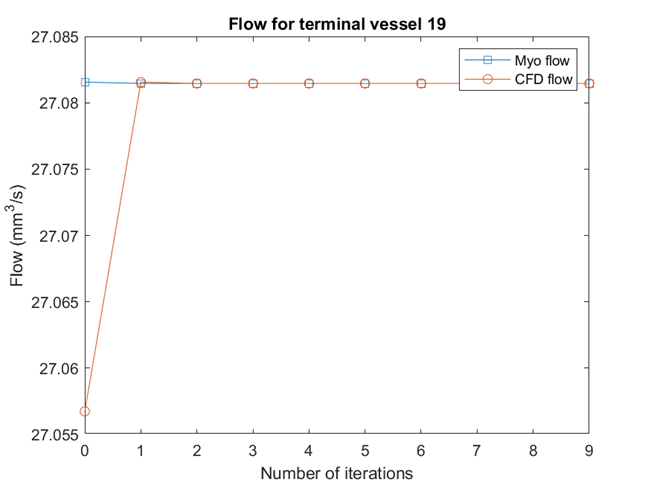
\includegraphics[width = 0.55\textwidth]{Fig/Results/Case1/Flow19.png}}
\hspace{0.1cm}
\subfloat{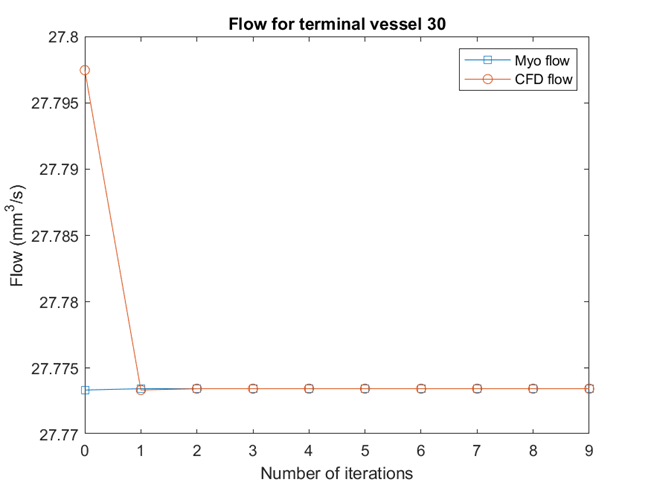
\includegraphics[width = 0.55\textwidth]{Fig/Results/Case1/Flow30.png}}
\caption{Flow results along iterations at terminal segments $15$ and $30$ in case 1.}
\label{fig:flcase1}
\end{center}
\end{adjustwidth}
\end{figure*}

\begin{figure}[hbtp]
\begin{center}

\subfloat[\label{pr1crv}]{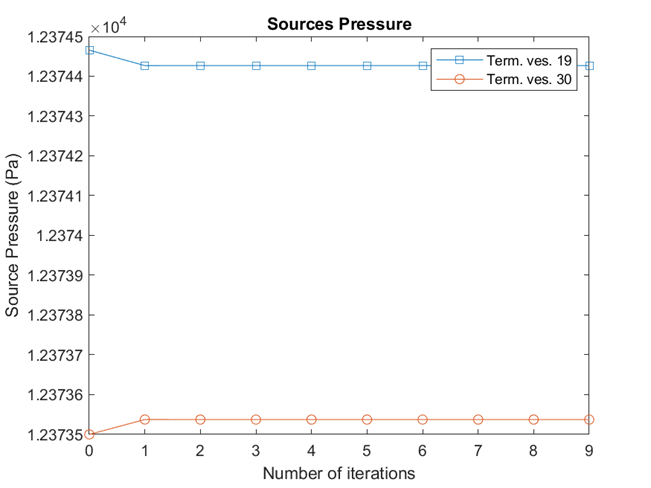
\includegraphics[width = 0.55\textwidth]{Fig/Results/Case1/Pressure.png}}
\subfloat[\label{pr1visu}]{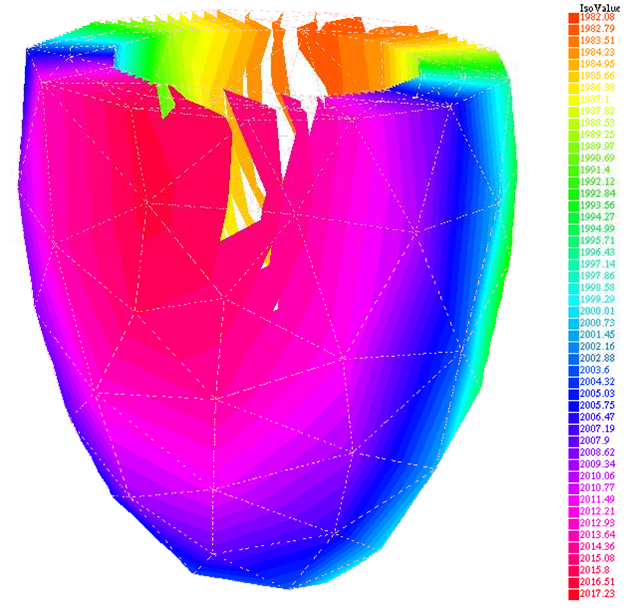
\includegraphics[width = 0.5\textwidth]{Fig/Results/Case1/FreefemPressure.png}}
\caption{Pressure results in case 1. \protect\subref{pr1crv} Pressure along iterations at terminal segments $15$ and $30$ in case 1. \protect\subref{pr1visu} Visualization of pressure iso values in porous model at iteration $9$}
\label{fig:prcase1}
\end{center}
\end{figure}


\subsubsection{Results for case $3$}
The case $3$ corresponds to an unequal diameter bifurcation in rest condition. However the associated territory to each terminal segment $\Omega_i$ are still equivalent, as in case 1. 
The table \ref{tab:case3} summarizes the initial parameters.
\begin{figure}[hbtp]
\begin{adjustwidth}{-3.5cm}{}
  \begin{center}
  	\caption{Initial parameters for case 3}
    \label{tab:case3}   
    \begin{tabular}{c|c|c|c|l}  
      \textbf{Parameter} & \multicolumn{2}{c|}{\textbf{Value}} &  \textbf{Units} & \textbf{Description}     \\
      \hline
      $K$           & \multicolumn{2}{c|}{$0.002$}     & \si{mm^{2}.Pa^{-1}.s^{-1}}    & Permeability div$.$ by blood viscosity   \\
      $P_{sink}$     & \multicolumn{2}{c|}{$0$}          & \si{\Pa}     & Venous tree pressure     \\
      $\beta_{sink}$ & \multicolumn{2}{c|}{\SI{10.1821e-4}{}}  & \si{Pa^{-1}.s^{-1}} & Venous tree beta           \\
      $\bar{P}$     & \multicolumn{2}{c|}{$1999.84$}    & \si{\Pa}      & Average capillary tree pressure    \\      
      \hline
      \hline
                    & \textbf{tv 19} & \textbf{tv 30} &         &                                              \\
      \hline
      $P_{source,k=0}^{i}$       & \SI{12353.1806}{} & \SI{12394.3465}         & Pa      & Source pressure for term$.$ vessel $i$              \\
      $\beta_{source}^{i}$   & \SI{3.1116e-5} & \SI{1.1107e-5}   & \si{Pa^{-1}.s^{-1}} &  Beta of term$.$ vessel $i$  \\
      $q^{T,i}_{k=0}$       & \SI{40.5528} & \SI{14.3013}           & \si{mm^3.s^{-1}}  & Flow rate of term$.$ vessel $i$                  \\               
      $R^{T,i}_{k=0}$       & \SI{304.619} & \SI{862.2408}               & \si{\Pa  \per\cubic\milli\meter \second}       & Resistance of term$.$ vessel $i$                           \\
      $V_{perf}^{i}$       & \SI{126.5640} & \SI{123.1915}                & \si{\cubic\milli\meter}    & Perfusion volume of term$.$ vessel $i$                \\
     
    \end{tabular}
  \end{center}
\end{adjustwidth}
\end{figure}

The figures \ref{fig:flcase3} and \ref{fig:prcase3}\protect\subref{prcurve} show respectively flow and pressure evolution at terminal segment outlets along iterations. The simulation requires one more iteration than in case 1 to converge, which can be expected since the bifurcation is unbalanced. The pressures converged to their final values at the third iteration, and flow values are exactly equal at the next one. 
The figure \ref{fig:prcase3}\protect\subref{prvisu} provides visualization of the iso pressure in the porous model at the 9th iteration, so reached convergence. The pressure values obtained in myocardium show a larger range than in case 1: minimum and maximum are respectively \SI{1605.75}{} and \SI{2360.15}{Pa}, corresponding to \SI{12.04}{} and \SI{17.70}{\mmHg}. 

\begin{figure*}[hbtp]
\begin{adjustwidth}{-2cm}{}
\begin{center}
\subfloat{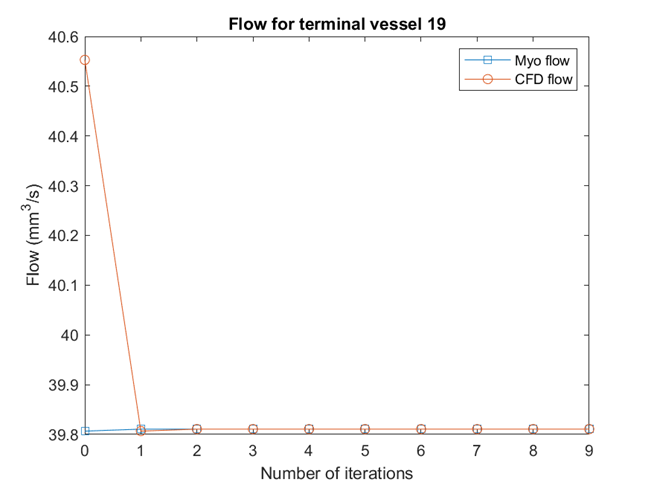
\includegraphics[width = 0.55\textwidth]{Fig/Results/Case3/Flow19.png}}
\hspace{0.1cm}
\subfloat{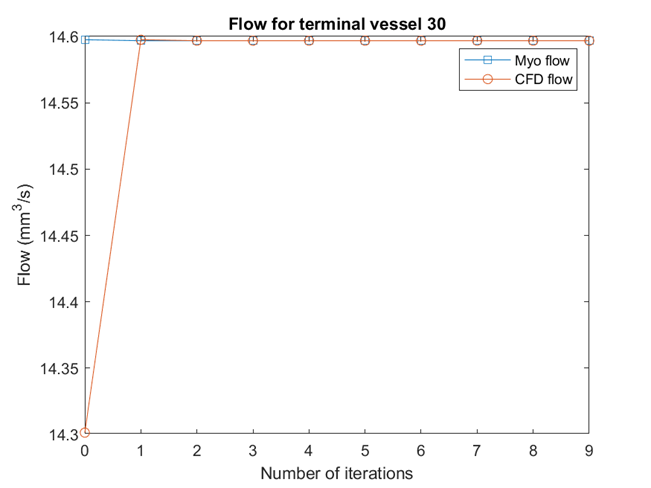
\includegraphics[width = 0.55\textwidth]{Fig/Results/Case3/Flow30.png}}
\caption{Flow results along iterations at terminal segments $19$ and $30$ in case 3.}
\label{fig:flcase3}
\end{center}
\end{adjustwidth}
\end{figure*}

\begin{figure}[hbtp]
\begin{center}
\subfloat[\label{prcurve}]{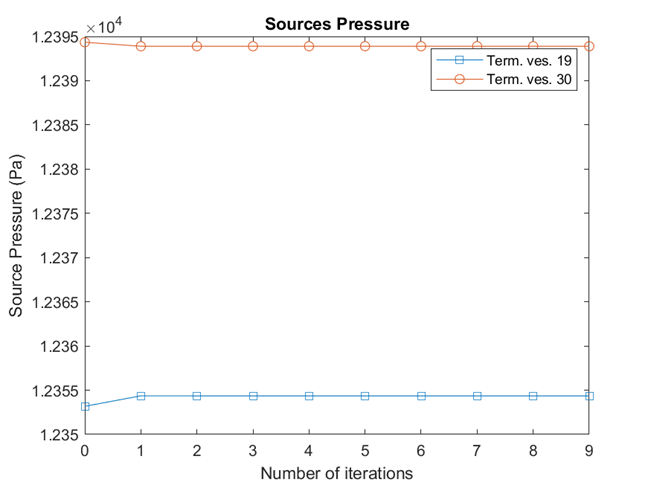
\includegraphics[width = 0.55\textwidth]{Fig/Results/Case3/Pressure.png}}
\subfloat[\label{prvisu}]{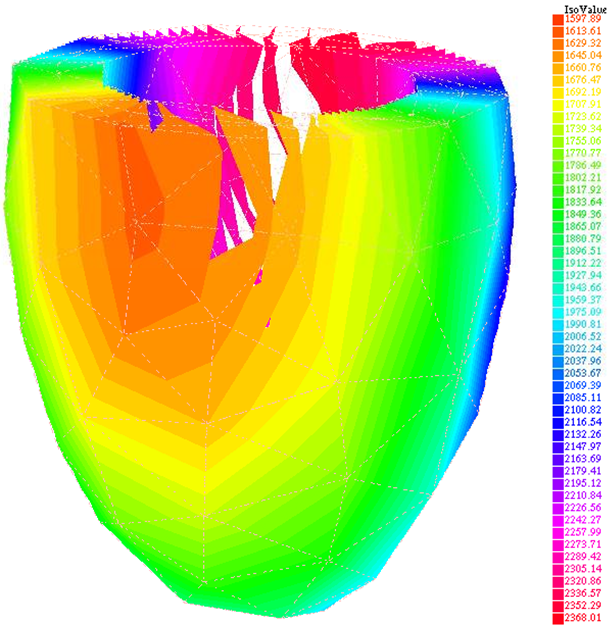
\includegraphics[width = 0.5\textwidth]{Fig/Results/Case3/FreefemPressure.png}}
\caption{Pressure results in case 3. \protect\subref{prcurve}: along iterations at terminal segments $15$ and $19$. \protect\subref{prvisu}:Visualization of pressure iso values in porous model at iteration $9$.}
\label{fig:prcase3}
\end{center}
\end{figure}

\subsubsection{Results for case $6$}

The cases $6$ challenges the porous model properties by imposing equal $\beta_{source}$ values for an unequal diameter bifurcation, in rest condition. With this parameterization we expect convergence to be achieved with equal flow values at terminal vessels.

The table \ref{tab:case6} summarizes the initial parameters.
\begin{figure}[hbtp]
\begin{adjustwidth}{-3.5cm}{}
  \begin{center}
  	\caption{Initial parameters for case 6}
    \label{tab:case6}   
    \begin{tabular}{c|c|c|c|l}  
      \textbf{Parameter} & \multicolumn{2}{c|}{\textbf{Value}} &  \textbf{Units} & \textbf{Description}     \\
      \hline
      $K$           & \multicolumn{2}{c|}{$0.002$}     & \si{mm^{2}.Pa^{-1}.s^{-1}}    & Permeability div$.$ by blood viscosity   \\
      $P_{sink}$     & \multicolumn{2}{c|}{$0$}          & \si{\Pa}     & Venous tree pressure     \\
      $\beta_{sink}$ & \multicolumn{2}{c|}{\SI{10.8935e-5}{}}  & \si{Pa^{-1}.s^{-1}} & Venous tree beta           \\
      $\bar{P}$     & \multicolumn{2}{c|}{$1999.84$}    & \si{\Pa}      & Average capillary tree pressure    \\      
      \hline
      \hline
                    & \textbf{tv 19} & \textbf{tv 30} &         &                                              \\
      \hline
      $P_{source,k=0}^{i}$       & \SI{12353.1806}{} & \SI{12394.3465}         & Pa      & Source pressure for term$.$ vessel $i$              \\
      $\beta_{source,homogeneous}^{i}$   & \SI{2.1e-5} & \SI{2.1e-5}   & \si{Pa^{-1}.s^{-1}} &  Beta of term$.$ vessel $i$  \\
      $q^{T,i}_{k=0}$       & \SI{40.5528} & \SI{14.3013}           & \si{mm^3.s^{-1}}  & Flow rate of term$.$ vessel $i$                  \\               
      $R^{T,i}_{k=0}$       & \SI{304.619} & \SI{862.2408}               & \si{\Pa  \per\cubic\milli\meter \second}       & Resistance of term$.$ vessel $i$                           \\
      $V_{perf}^{i}$       & \SI{126.5640} & \SI{123.1915}                & \si{\cubic\milli\meter}    & Perfusion volume of term$.$ vessel $i$                \\
    \end{tabular}
  \end{center}
\end{adjustwidth}
\end{figure}

The figures \ref{fig:flcase6} and \ref{fig:prcase6}\protect\subref{prcurve} show respectively flow and pressure evolution at terminal segment ends along iterations.  
Pressure and flow convergence are reached at same iteration as in case $3$. As expected, converged terminal flow values are equal despite the unbalanced diameter bifurcation. Also, the terminal segment end pressures converge toward close values, respectively \SI{12373.89} and \SI{12374.76}{\Pa} for vessel $19$ and $30$. The resulting pressure field in the myocardium is nearly constant: only a \SI{4e-2}{\Pa} drop, see figure \ref{fig:prcase3}\protect\subref{prvisu}. These results show the homogenization impact of the porous model on the whole simulation. 


\begin{figure*}[hbtp]
\begin{adjustwidth}{-2cm}{}
\begin{center}
\subfloat{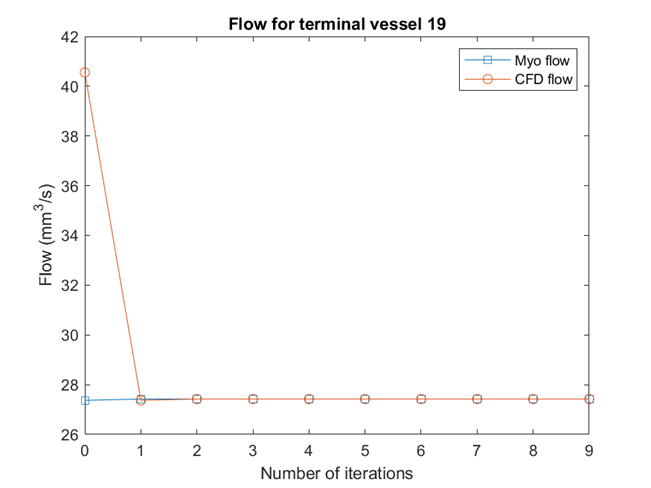
\includegraphics[width = 0.55\textwidth]{Fig/Results/Case6/Flow19.png}}
\hspace{0.1cm}
\subfloat{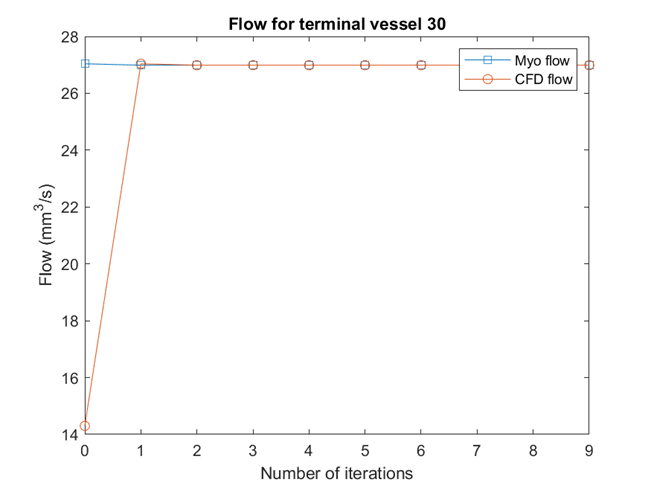
\includegraphics[width = 0.55\textwidth]{Fig/Results/Case6/Flow30.png}}
\caption{Flow results along iterations at terminal segments $19$ and $30$ in case 6.}
\label{fig:flcase6}
\end{center}
\end{adjustwidth}
\end{figure*}

\begin{figure}[hbtp]
\begin{center}
\subfloat[\label{prcurve}]{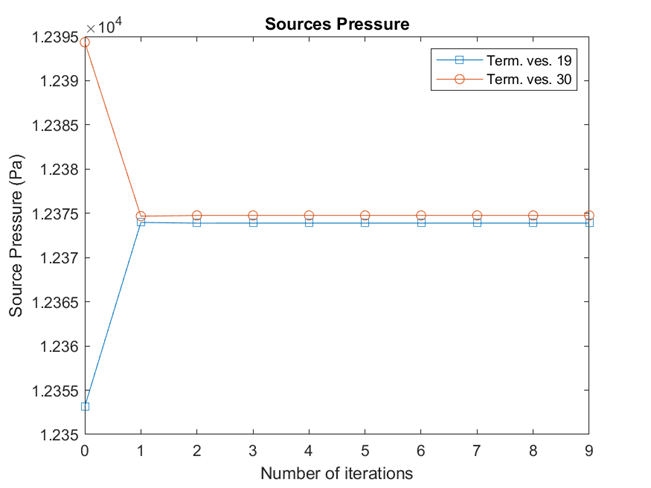
\includegraphics[width = 0.55\textwidth]{Fig/Results/Case6/Pressure.png}}
\subfloat[\label{prvisu}]{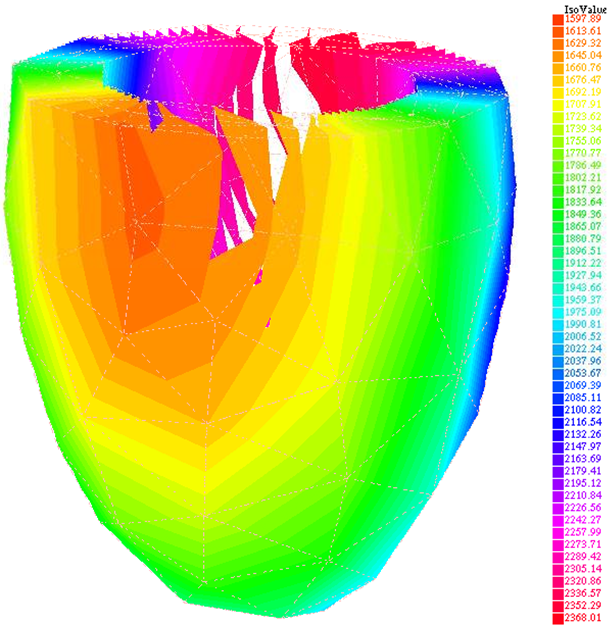
\includegraphics[width = 0.5\textwidth]{Fig/Results/Case3/FreefemPressure.png}}
\caption{Pressure results in case 6. \protect\subref{prcurve}: along iterations at terminal segments $19$ and $30$. \protect\subref{prvisu}:Visualization of pressure iso values in porous model at iteration $9$.}
\label{fig:prcase6}
\end{center}
\end{figure}



\subsubsection{Summary of results on simulated data}
All case results are summarized in table \ref{tab:rescase}.
The coupling results show communication between the two models, and convergence within $2-3$ iterations for all cases.

Results obtained in stress conditions exhibit both higher terminal segment flows, and higher pressure drop in the myocardium, which is coherent.

Case $5$ and $6$ highlight the impact of porous model $\beta_{source}$ parameterization on the coupling. Unequal values induce differenciation of terminal segment flow and higher pressure drop inside the myocardium. Equal value on whole myocardium is responsible for homogenization of terminal segment flow and myocardium pressure drop decrease.
\begin{figure}[hbtp]
\begin{adjustwidth}{-2.8cm}{}
\begin{center}
\begin{tabular}{|p{3.5cm}|p{3cm}|p{3cm}|p{4.5cm}|}
\hline
 & Rest & Stress & Rest with homogeneous $\beta$\\
 \hline
 Equal diameter & case $1$ & case $2$ & case 5: unequal $\beta_{source}^i$ ($\sim$case $3$ values)\\
\hdashline
$q^{T,19}$ (\si{\cubic\milli\meter\per\second})	& $27.08$ &   $106.90$ & $39.81$ \\
$q^{T,30}$ (\si{\cubic\milli\meter\per\second})	& $27.77 $ &  $109.40$ & $14.60$ \\
$\Delta P_{myo}$ (\si{\Pa})				& $34.43$ & $61.57$ & $754.40$ \\
 \hline
 Unequal diameter & case $3$ & case $4$ & case 6: equal $\beta_{source}^i$ ($\sim$case 1 values)\\
 \hdashline
 $q^{T,19}$ (\si{\cubic\milli\meter\per\second})	& $39.81$ &   $153.07$ & $27.42$ \\
$q^{T,30}$ (\si{\cubic\milli\meter\per\second})	& $14.60$ &  $59.60$ & $26.99$ \\
$\Delta P_{myo}$ (\si{\Pa})				& $754.40$ & $1336.72$ & $0.06$ \\
 \hline
\end{tabular}
\caption{Definition of the $6$ cases studied.}
\label{tab:rescase}
\end{center}
\end{adjustwidth}
\end{figure}

\subsection{Preliminary result on patient data}
We obtained a preliminary result on patient data. This result corresponds to a $1$ way coupling, meaning at the end of the step $k=0$. It was computed in rest condition for two different definition of the $\beta_{source}$ parameters.

In the case (i) we calculate the $\beta_{source}$ as described in \ref{subsec:parameter}, we obtain minimum and maximum pressure value inside the myocardium respectively of \SI{10.16} and \SI{23.07}{\mmHg}, see figure \ref{fig:pat_casei}.
In the case (ii), we use a single $\beta_{source}$ for the whole myocardium, of value \SI{3e-6}{\per\Pa\per\second}. We obtain a smaller pressure drop inside the myocardium, with minimum and maximum pressure value respectively of \SI{14.69} and \SI{15.49}{\mmHg}, see figure \ref{fig:pat_caseii}.

\begin{figure*}[hbtp]
\begin{adjustwidth}{-2cm}{}
\begin{center}
\subfloat{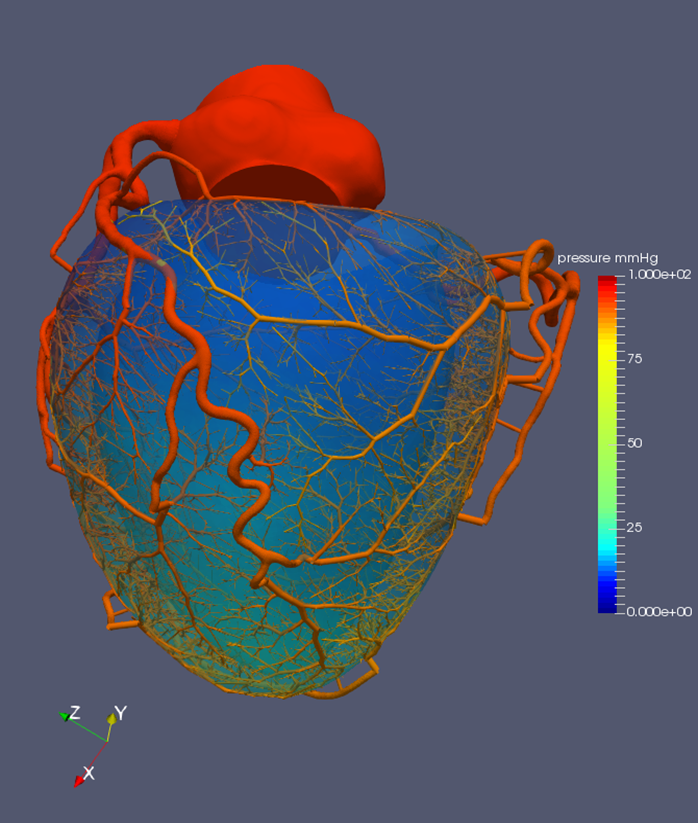
\includegraphics[width = 0.44\textwidth]{Fig/PatientResults/Case1_visu2.png}}
\hspace{0.05cm}
\subfloat{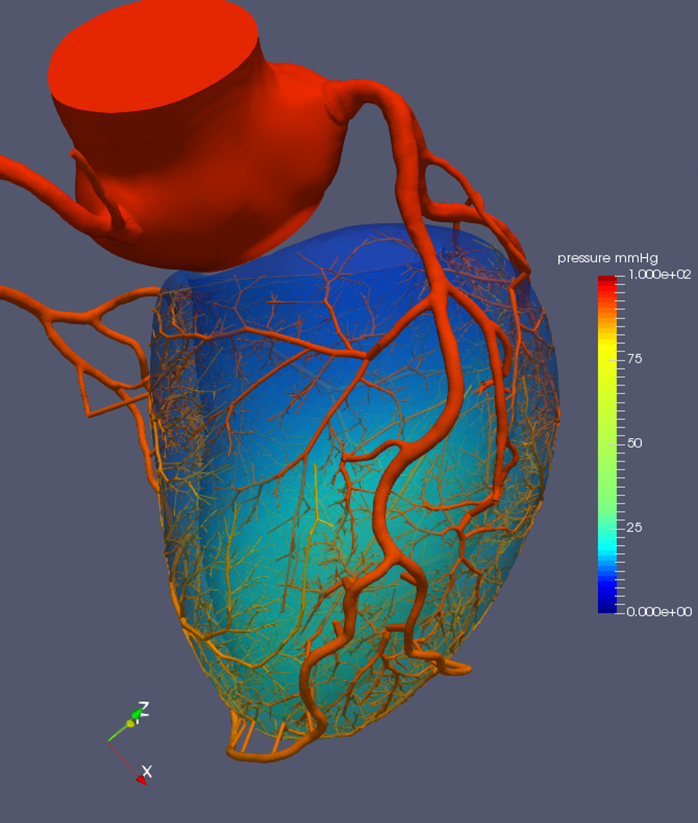
\includegraphics[width = 0.44\textwidth]{Fig/PatientResults/Case1_visu1.png}}
\caption{Pressure results of the 1 way coupling on case (i) for 1 patient}
\label{fig:pat_casei}
\end{center}
\end{adjustwidth}
\end{figure*}

\begin{figure*}[hbtp]
\begin{adjustwidth}{-2cm}{}
\begin{center}
\subfloat{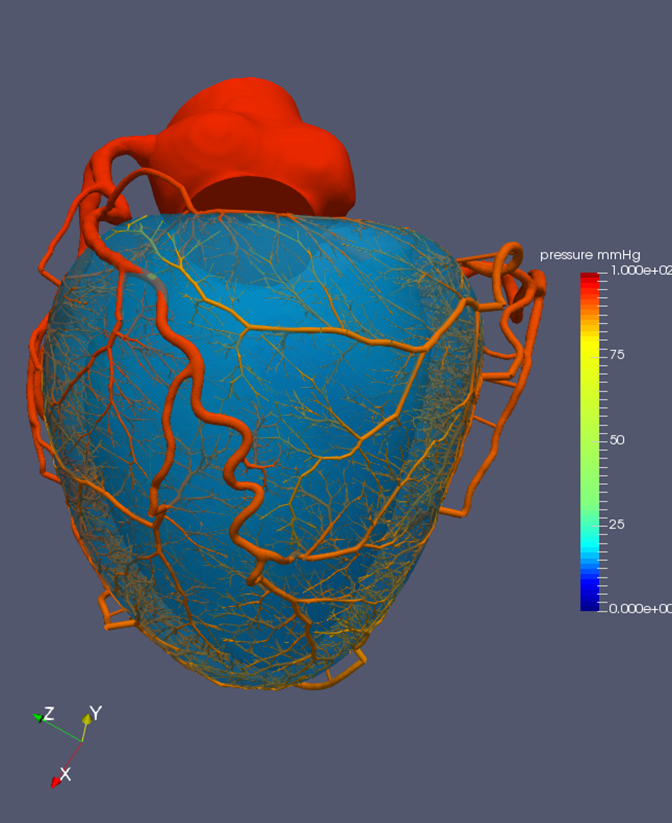
\includegraphics[width = 0.44\textwidth]{Fig/PatientResults/Case2_visu2.png}}
\hspace{0.05cm}
\subfloat{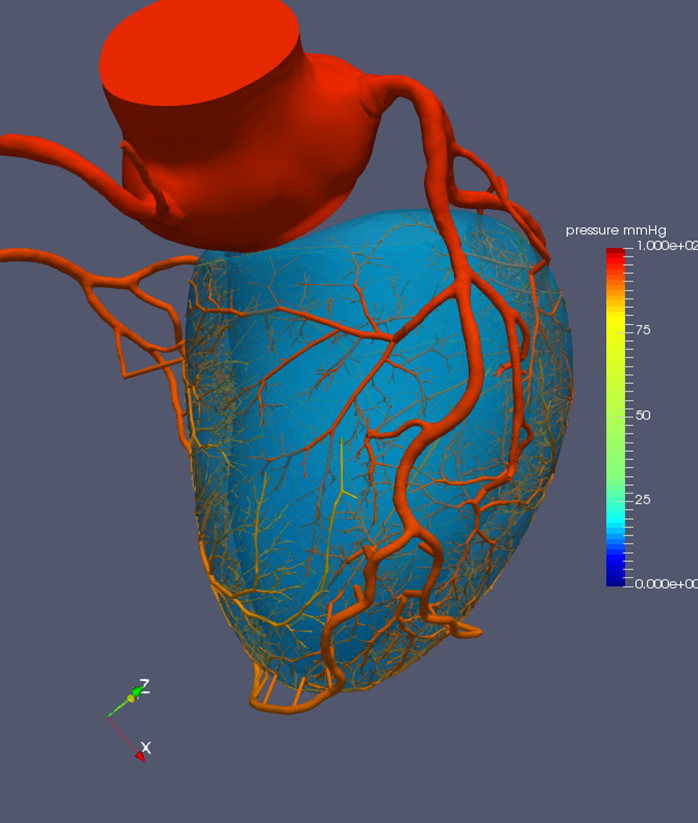
\includegraphics[width = 0.44\textwidth]{Fig/PatientResults/Case2_visu1.png}}
\caption{Pressure results of the 1 way coupling on case (ii) for 1 patient}
\label{fig:pat_caseii}
\end{center}
\end{adjustwidth}
\end{figure*}
 

Technical issues need to be resolved, and these results will be submitted to further investigations. We are also working on implementation of the last step of the loop.


\section{Future work}

The final objective is to assess this coupling on patient data: with the $6000$ terminal segment generated network, and our left ventricle segmentation.
It will be interesting to compare with the flow distribution obtained in Clara thesis chapter 8 section 5. We expect the coupling to induce homogenization of the flow distribution. 



Parameterization of both coronary and porous model can be studied in regard of the ground-truth data. In particular $\beta_{source}$ can be estimated locally, globally, or interpolated via the distance to the source term. 

Also, the coupling could be assessed on vascular network of various size (number of terminal segments), to identify the adequate size that enables to reach flow homogenization.
In order to confirm the parameterization of the coupled modelization, we will also need to assess it on patient data with acute disease.


%----------------------------------------------------------------------------------------
%	BIBLIOGRAPHY
%----------------------------------------------------------------------------------------

\bibliographystyle{unsrt}

\bibliography{sample}

%----------------------------------------------------------------------------------------

\end{document}